\documentclass{beamer}
\usepackage[british,spanish]{babel}
\usepackage[utf8]{inputenc}

\usepackage{hyperref}
%\hypersetup{colorlinks=false,linkbordercolor=red,linkcolor=green,pdfborderstyle={/S/U/W 1}}

\usepackage{multirow}

\usepackage{textcomp}

\usepackage{listings}
\lstloadlanguages{Ruby}

\usepackage{adjustbox}
\usepackage{lstcustom}

\usepackage{amsmath}

\usepackage{color}
\definecolor{light-gray}{gray}{0.80}
\definecolor{lstbackgroundshellcolor}{named}{light-gray}

\usepackage{tikz}
\newcommand*\circled[1]{\tikz[baseline=(char.base)]{
            \node[shape=circle,draw,inner sep=2pt] (char) {#1};}}

\usepackage[normalem]{ulem}

%\usepackage[acronym,xindy,toc]{glossaries}

\usepackage[acronym,xindy,toc]{glossaries}
\makeglossaries
%\usepackage[xindy]{imakeidx}
%\makeindex


\newcommand{\comment}[2]{#2}

\newcommand{\commandinline}[1]{\lstinline[basicstyle=\small\lstfontfamily]{#1}}
\newcommand{\outputcommand}[1]{\color{darkgreen}{#1}}

\graphicspath{ {./images/} }

\title{Deploying a Ruby on Rails Application in an Amazon EC2 Virtual Machine}
%\subtitle[short subtitle]{long subtitle}
\author[C. Cuenca, F. Quintana]{Carmelo Cuenca-Hernández and Francisca Quintana-Domínguez}
%\institute{Escuela Universitaria de Informática}
%\date[04/2013]{Abril - 2013}
\date{}
\titlegraphic{
\includegraphics[width=0.5 \textwidth]{./images/logo_ulpgc_version_horizontal_rgb.eps}}



\pgfdeclareimage[width=2.0\baselineskip]{ulpgc-logo}{./images/logosimbolo_secundario_version_vertical}
\setbeamertemplate{footline}{\raisebox{-2ex}{\pgfuseimage{ulpgc-logo}}
  \usebeamerfont{date in head/foot}\insertshortdate{}\hfill
  \usebeamertemplate{navigation symbols}\hfill
  \insertframenumber{}/\inserttotalframenumber}
\setbeamertemplate{sidebar right}{}


\usetheme{Antibes}
%\usetheme{Berlin}

%\usetheme{Warsaw}
%\usecolortheme{albatross}

\selectlanguage{british}

\begin{document}


\begin{frame}
	\titlepage
\end{frame}


\section*{Outline}
\begin{frame}
  \frametitle{Outline}
  %\tableofcontents%[part=1,pausesections]
  \tableofcontents[currentsection,currentsubsection, sectionstyle=show] 
  %\tableofcontents[currentsection,sectionstyle=show,hideothersubsections]
\end{frame}

%%%%%%%%%%%%%%%%%%%%%%%%%%%%%%%%%%%%%%%%%%%%%%%%%%%%%%%%%%%%%%%%%%%%%%%%%%%%%%
%\newacronym{<label>}{<abbrv>}{<full>}
%\glsreset{<label>}
%\glsresetall
%\acrlong{<label>}
%\acrfull{<label>}
%\acrshort{<label>}
%\input{../glossary}

\newacronym{aws}{AWS}{Amazon Web Services}
\newacronym{css}{CSS}{cascading style sheets}
\newacronym{ebs}{EBS}{Elastic Block Storage}
\newacronym{ec2}{EC2}{Amazon Elastic Compute Cloud}
\newacronym{elb}{ELB}{Elastic Load Balancing}
\newacronym{ror}{RoR}{{\href{http://rubyonrails.org/}{Ruby on Rails}}}
\newacronym{rds}{RDS}{Relational Database Service}
\newacronym{rvm}{RVM}{{\href{https://rvm.io/}{Ruby Version Manager}}}
\newacronym{s3}{S3}{Simple Storage Service}
\newacronym{sqs}{SQS}{Amazon Simple Queue Service}
%%%%%%%%%%%%%%%%%%%%%%%%%%%%%%%%%%%%%%%%%%%%%%%%%%%%%%%%%%%%%%%%%%%%%%%%%%%%%%
%%%%%%%%%%%%%%%%%%%%%%%%%%%%%%%%%%%%%%%%%%%%%%%%%%%%%%%%%%%%%%%%%%%%%%%%%%%%%%
%\section*{Web Server in Production Mode}

\begin{frame}[fragile, allowframebreaks]
\frametitle{Web Server in Production Mode}
Amazon es el mayor proveedor de servicios para la ``nube'' en el mundo muy por delante de Google o Microsoft.
\acrfull{ec2} es uno de estos servicios y proporciona infraestructuras tecnológicas de computadores y posibilita
desplegar un computador a medida en la ``nube'' (una instancia de una imagen en lenguaje de Amazon)

\begin{itemize}
\item Nosotros desplegaremos una máquina ``micro'' con un CentOS 6.
Dado que esta máquina constituirá infraestructura para un entorno de producción, la imagen sólo contendrá inicialmente los paquetes mínimos (no Gnome, no KDE, no \dots).

\item Añadiremos los paquetes necesarios para convertirla en un servidor LAMP (Linux, Apache, MySQL y PHP) y configuraremos los diferentes cortafuegos: ``Security Groups'' de Amazon y SElinux de CentOS.
Testearemos el funcionamiento del servidor LAMP y aprovecharemos para introducir el concepto de ``Elastic IP'' (otro servicio de Amazon).

\item Dado que nuestra elección para el almacenamiento de datos no es MySQL, sino PostgreSQL (entre otras, por  razones de escalabilidad), convertiremos nuestra máquina en un servidor de PostgreSQL.

\item A continuación, portaremos una aplicación ya desarrollada en \acrfull{ror} que simula el código de cualquier aplicación. El éxito del despliege depende de configurar la máquina y convertirla en un servidor de aplicaciones \acrshort{ror}.
La metodología consiste en añadir primeramente un usuario para cada aplicación, limitando así los accessos a los recursos de la máquina (queremos tener múltiples aplicaciones en el mismo servidor).

\item Mediante \acrfull{rvm} instalaremos Ruby y \acrshort{ror}. Con ``Git''  colocaremos el código en la máquina virtual. Comprobaremos que funciona en los entornos de test y desarrollo.

\item Ya sólo nos faltará desplegar  un servidor porfesional de \acrshort{ror}, nuestra elección para ilustrar ha sido el más complejo de configurar ``unicorn''. Instalaremos Unicorn, comprobarmeos que funciona en el entorno de produción y escribiremos un script para lanzarlo como un servicio.

\item Finalmente, el alumno desarrollará un trabajo similar de desplegar cualquier otra aplicación \acrshort{ror} con cualquier otro servidor profesional (Passenger, Thin, Mogol).

\end{itemize}
\end{frame}

\section{Lauching an Amazon EC2 Instance}
\begin{frame}[fragile, allowframebreaks]
\frametitle{Lauching an Amazon EC2 Instance}

\begin{itemize}
\item Prepare a Key Pair
\item Edit ``Security Group'' 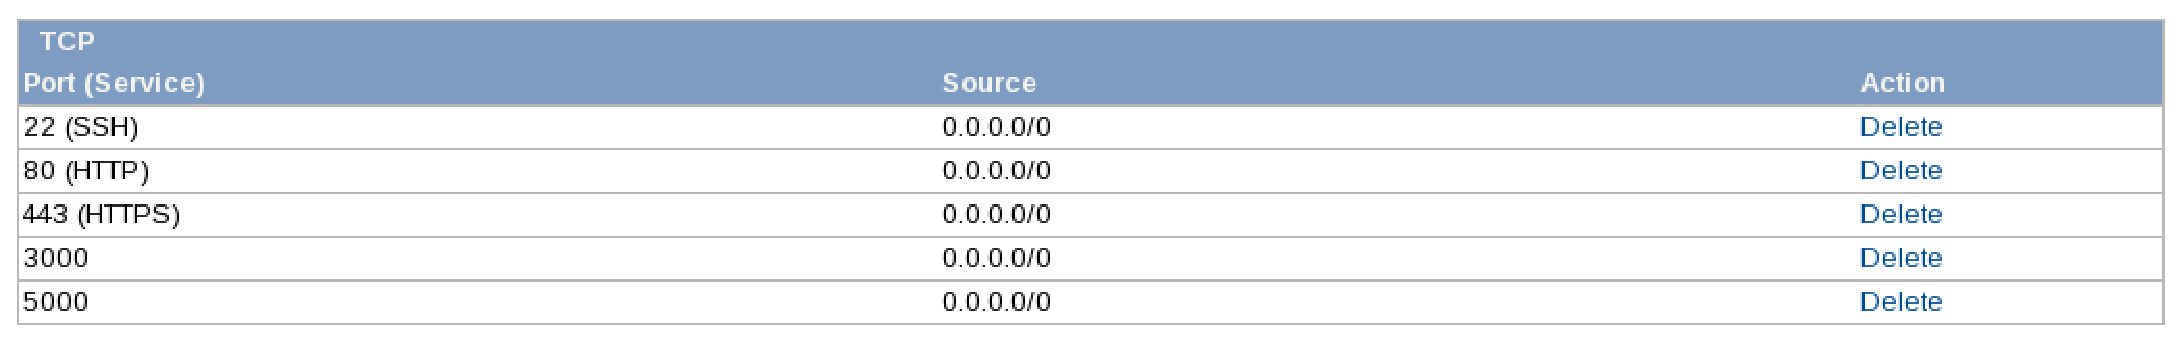
\includegraphics[width=1.0 \textwidth]{securitygroup.eps}
\item Launch a minimal \texttt{CentOS 6 (i386) - with Updates} in \url{https://aws.amazon.com/marketplace/pp/B00A6KZBC6/ref=sp_mpg_product_title?ie=UTF8&sr=0-2}
\item Then, we can login in the instance

\lstset{language=shell, escapechar=!}
\begin{lstlisting}[escapechar=!]
$ chmod 0600 your_key_file.pem 
$ ssh -i your_key_file.pem root@ec2-nnn-nnn-nn-nnn.compute-1.amazonaws.com
\end{lstlisting}

\end{itemize}

\end{frame}



%%%%%%%%%%%%%%%%%%%%%%%%%%%%%%%%%%%%%%%%%%%%%%%%%%%%%%%%%%%%%%%%%%%%%%%%%%%%%%



%%%%%%%%%%%%%%%%%%%%%%%%%%%%%%%%%%%%%%%%%%%%%%%%%%%%%%%%%%%%%%%%%%%%%%%%%%%%%%


\section{Installing a LAMP Web Server}
\begin{frame}[fragile, allowframebreaks]
\frametitle{Installing a LAMP Web Server}
\lstset{language=shell, escapechar=!}
\begin{itemize}
\item To ensure that all of your software packages are up to date, perform a quick software update on your instance
\begin{lstlisting}[escapechar=!]
# yum update -y
\end{lstlisting}
\item Now that your instance is updated, you can install the Apache web server, MySQL, and PHP software packages. Use the \texttt{yum groupinstall} command to install multiple software packages and all related dependencies at the same time
\lstset{language=shell}
\begin{lstlisting}[escapechar=!]
# export LANG=en_EN.utf8
# yum groupinstall -y "Web Server" "MySQL Database" "PHP Support"
\end{lstlisting}
\item Install the php-mysql package
\begin{lstlisting}[escapechar=!]
# yum install -y php-mysql
\end{lstlisting}

\item Start the Apache web server

\lstset{language=shell}
\begin{lstlisting}[escapechar=!]
# service httpd start
!\outputcommand{Starting httpd:                                            [  OK  ]}
\end{lstlisting}

\item Use the \texttt{chkconfig} command to configure the Apache web server to start at each system boot
\lstset{language=shell}
\begin{lstlisting}[escapechar=!]
# chkconfig httpd on
\end{lstlisting}

\item The \texttt{chkconfig} command does not provide any confirmation message when you successfully enable a service. You can verify that \texttt{httpd} is on by running the following command

\lstset{language=shell}
\begin{lstlisting}[escapechar=!]
# chkconfig --list httpd
!\outputcommand{httpd           0:off   1:off   2:on    3:on    4:on    5:on    6:off}
\end{lstlisting}

\item Modify the mode SELinux to permissive mode
\lstset{language=shell}
\begin{lstlisting}[escapechar=!]
# setenforce 0
\end{lstlisting}

\item Modify \texttt{/etc/selinux/config} to disable SELinux

\lstset{language=shell}
\begin{lstlisting}[escapechar=!]
# /etc/selinux/config
!\vdots!
SELINUX=disabled !\circled{1}!
!\vdots!
\end{lstlisting}

\item We use \texttt{system-config-firewall-tui} command to configure the firewall on your instance to allow these connections. 
Since \texttt{newt-python} is required for \texttt{system-config-firewall-tui to work}, it should be added to the AMI

(\href{http://bugs.centos.org/view.php?id=6877}{http://bugs.centos.org/view.php?id=6877})
\lstset{language=shell}
\begin{lstlisting}[escapechar=!]
# yum -y install newt-python 
# system-config-firewall-tui
\end{lstlisting}

\item We should open \texttt{http} port 80, \texttt{https} port 447,  \texttt{ssh} port 22 and \texttt{\alert{3000 and 5000}} ports for ``tcp'' protocol
 
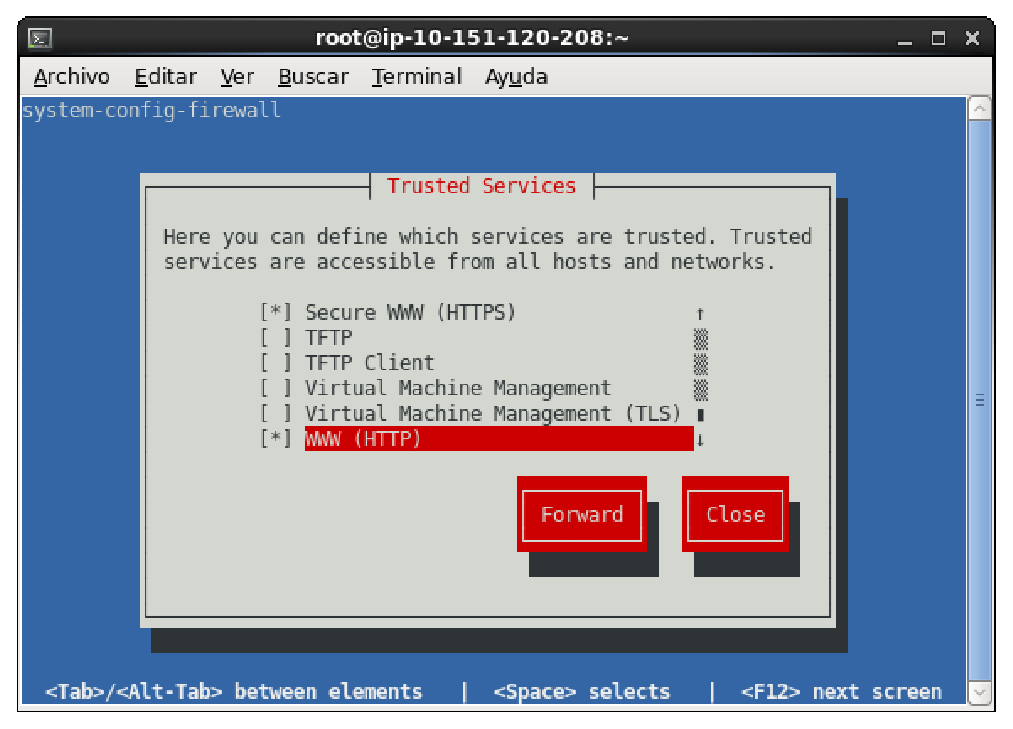
\includegraphics[width=0.5 \textwidth]{system-config-firewall-tui.eps}

\item To test your LAMP web server in a web browser,  create simple html and PHP files in the \texttt{/var/www/html} directory that will be available from the Internet with
\lstset{language=shell}
\begin{lstlisting}[escapechar=&]
# echo `<p>Hello World!<p>' > /var/www/html/index.html
# echo "<?php phpinfo(); ?>" > /var/www/html/phpinfo.php
\end{lstlisting}


\item Curl the URL of the files you just created. This URL is the public DNS address of your instance followed by a forward slash and the file name. For example
\lstset{language=shell}
\begin{lstlisting}[escapechar=!]
$ curl http://my.public.dns.amazonaws.com/
$ curl http://my.public.dns.amazonaws.com/phpinfo.php
\end{lstlisting}


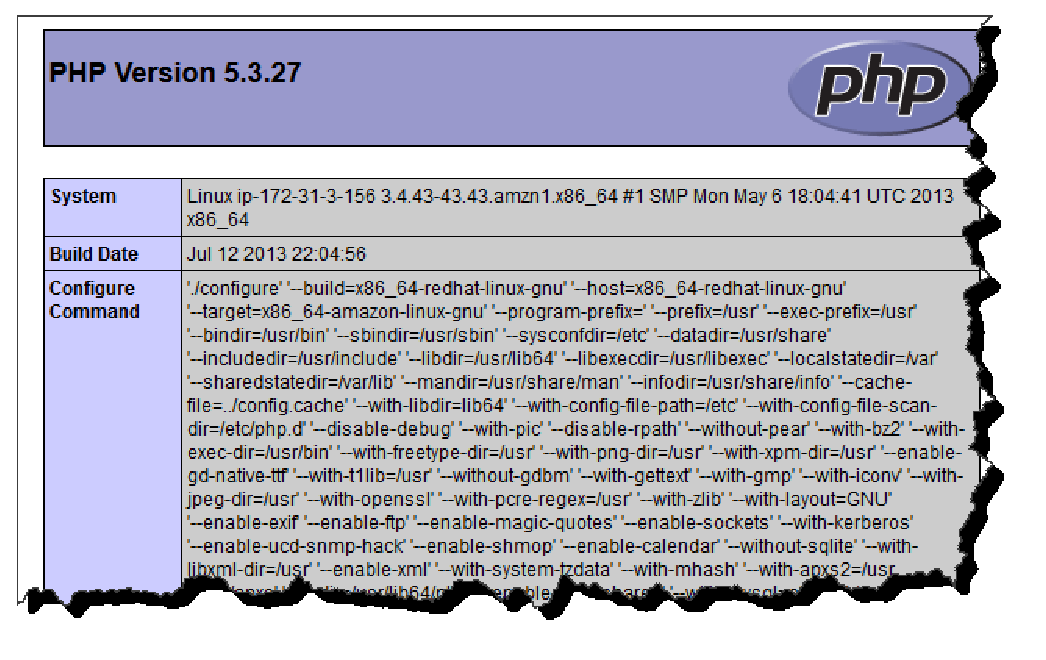
\includegraphics[width=0.5 \textwidth]{phpinfo.eps}

\item Delete the \texttt{phpinfo.php} file. Although this can be useful information to you, for security reasons it should not be broadcasted to the Internet

\lstset{language=shell}
\begin{lstlisting}[escapechar=&]
# rm /var/www/html/phpinfo.php
\end{lstlisting}

\end{itemize}
\end{frame}
\begin{frame}[fragile,allowframebreaks]
\frametitle{UserDir }
\begin{itemize}
 \item Edit the file \texttt{/etc/httpd/conf/httpd.conf} in order to enable requests to \texttt{/\char126user/} to serve the user's \texttt{public\_html}



\lstset{language=shell,numbers=left}
\begin{lstlisting}[escapechar=!]
!\vdots!
<IfModule mod_userdir.c>
!\vdots!
    # UserDir disabled !\circled{1}!
    UserDir enabled *
    UserDir disabled root
!\vdots!
    # !\circled{2}!
    UserDir public_html

</IfModule>

!\vdots!
<Directory /home/*/public_html>
    AllowOverride FileInfo AuthConfig Limit
    Options MultiViews Indexes SymLinksIfOwnerMatch IncludesNoExec
    <Limit GET POST OPTIONS>
        Order allow,deny
        Allow from all
    </Limit>
    <LimitExcept GET POST OPTIONS>
        Order deny,allow
        Deny from all
    </LimitExcept>
</Directory>
\end{lstlisting}

\item Restart Apache web server

\lstset{language=shell}
\begin{lstlisting}[escapechar=&]
# /etc/init.d/httpd restart
\end{lstlisting}

\end{itemize}
\end{frame}
%%%%%%%%%%%%%%%%%%%%%%%%%%%%%%%%%%%%%%%%%%%%%%%%%%%%%%%%%%%%%%%%%%%%%%%%%%%%%%

\section{Building System}
\begin{frame}[fragile]
\frametitle{Build System}
\lstset{language=shell, escapechar=!}
\begin{itemize}
\item Installing wget
\begin{lstlisting}[escapechar=!]
# yum -y wget
\end{lstlisting}

\item Installing EPEL (Extra Packages for Enterprise Linux) repository 
\begin{lstlisting}[escapechar=!]
# cd /tmp
# wget "http://dl.fedoraproject.org/pub/epel/6/i386/epel-release-6-8.noarch.rpm"
# rpm -ivh epel-release-6-8.noarch.rpm
\end{lstlisting}

\item And some extras packages \dots

\begin{lstlisting}[escapechar=!]
# yum install -y yum-utils
# yum install -y patch gcc-c++ readline-devel zlib-devel libyaml-devel libffi-devel openssl-devel autoconf automake libtool bison
# yum install -y sqlite-devel
# yum install -y git
\end{lstlisting}
\end{itemize}
\end{frame}
%%%%%%%%%%%%%%%%%%%%%%%%%%%%%%%%%%%%%%%%%%%%%%%%%%%%%%%%%%%%%%%%%%%%%%%%%%%%%%
\section{A JavaScript Runtime (Node.js)}

\begin{frame}[fragile]
\frametitle{A JavaScript Runtime (Node.js)}
\begin{columns}
  \column{ 0.15 \textwidth}
    \href{http://nodejs.org/}{
\includegraphics[width = 1.0 \textwidth]{nodejs.eps}}
  
    \url{http://nodejs.org/}
  \column{ 0.85 \textwidth}
  \begin{itemize}
   \item \texttt{Node.js} is a platform built on Chrome's JavaScript runtime for easily building fast, scalable network applications
   \lstset{language=shell, escapechar=!}
\begin{lstlisting}[escapechar=!]
# yum -y install nodejs
\end{lstlisting}
  \end{itemize}
\end{columns}


\end{frame}

\section{PostgresSQL}
\begin{frame}[fragile]
\frametitle{PostgresSQL}

\begin{columns}
\column{0.20 \textwidth}
\href{http://www.postgresql.org/}{
\includegraphics[width=0.75 \textwidth]{postgreSQL300x300.eps}}
 \url{http://www.postgresql.org/}
\column{0.80 \textwidth}
\begin{itemize}
  \item ``The world's most advanced open source database''
  \item Main PostgreSQL features include the following:
  \begin{itemize}
    \item Transactions
    \item Subselects
    \item Views
    \item Foreign key referential integrity
    \item Sophisticated locking
    \item User-defined types
    \item Inheritance
    \item Rules
    \item Multiple-version concurrency control
  \end{itemize}

\end{itemize}
\end{columns}
\end{frame}



\begin{frame}[fragile, allowframebreaks]
\frametitle{PostgresSQL}
\begin{itemize}
\item Edit your distributions \texttt{.repo file} located \texttt{/etc/yum.repos.d/CentOS-Base.repo} and located the \texttt{[base]} and \texttt{[updates]} sections.
To the section(s) identified above, you need to append a line

\lstset{language=shell, escapechar=!,numbers=left}
\begin{lstlisting}[escapechar=!]
exclude=postgresql*
\end{lstlisting}

\item Download PGDG RPM file (Browse \url{http://yum.postgresql.org} and find your correct RPM)

\lstset{language=shell, escapechar=!}
\begin{lstlisting}[escapechar=!]
# cd /tmp
# curl -O http://yum.postgresql.org/9.3/redhat/rhel-6-i386/pgdg-centos93-9.3-1.noarch.rpm
\end{lstlisting}

\item Now install PGDG RPM  distribution

\begin{lstlisting}[escapechar=!]
# rpm -ivh pgdg-centos93-9.3-1.noarch.rpm
\end{lstlisting}

\lstset{language=shell, escapechar=!}
\begin{lstlisting}[escapechar=!]
$ yum list postgresql93-*
!\outputcommand{A lot of stuff}!
# yum groupinstall -y "PostgreSQL Database Server 9.3 PGDG"
# yum install -y postgresql93-devel phpPgAdmin
\end{lstlisting}

\item This \texttt{service} command (only needed once) is to initialize the database in PGDATA
 
\lstset{language=shell, escapechar=!}
\begin{lstlisting}[escapechar=!]
# ls /var/lib/pgsql/9.3/data/*
!\outputcommand{ls: cannot access /var/lib/pgsql/9.3/data/*: No such file or directory}!
\end{lstlisting}


\lstset{language=shell, escapechar=!}
\begin{lstlisting}[escapechar=!]
# service postgresql-9.3 initdb
!\outputcommand{Initializing database:                                     [  OK  ]}!
\end{lstlisting}

\lstset{language=shell, escapechar=!}Finally \dots
\begin{lstlisting}[escapechar=!]
# ls /var/lib/pgsql/9.3/data/*
!\outputcommand{A lot of stuff}!
\end{lstlisting}

\item Start the PostgreSQL Server

\lstset{language=shell, escapechar=!}
\begin{lstlisting}[escapechar=!]
# /etc/init.d/postgresql-9.3 start
!\outputcommand{Starting postgresql-9.3 service:                           [  OK  ]}!
# chkconfig postgresql-9.3 on
# chkconfig --list postgresql-9.3
!\outputcommand{postgresql-9.3 	0:off	1:off	2:on	3:on	4:on	5:on	6:off}!
\end{lstlisting}

\item Add PostgreSQL path to \texttt{\$PATH}

\lstset{language=shell, escapechar=!}
\begin{lstlisting}[escapechar=!]
# echo "export PATH=$PATH:/usr/pgsql-9.3/bin/" > /etc/profile.d/pgsql-9.3.sh
\end{lstlisting}

\item Create a role with name \texttt{depot\_app} which can create databases, can not create roles, is not superuser and needs a password

\lstset{language=shell, escapechar=!}
\begin{lstlisting}[escapechar=!]
# su - postgres
$ createuser -d -R -S -P depot_app
!\outputcommand{Enter password for new role:}!
!\outputcommand{Enter it again:}!
\end{lstlisting}

\item Edit the PostgreSQL configuration file \texttt{/var/lib/pgsql/9.3/data/pg\_hba.conf}

\lstset{language=shell, escapechar=!, numbers=left}
\begin{lstlisting}[escapechar=!]
!\vdots!
# "local" is for Unix domain socket connections only
local   all postgres peer !\circled{1}!
local   all all      md5  !\circled{2}!
# IPv4 local connections:
host    all all      127.0.0.1/32 md5 !\circled{3}!
# IPv6 local connections:
host    all all ::1/128 md5 !\circled{4}!
!\vdots!
\end{lstlisting}

\item Restart the PostgreSQL daemon

\lstset{language=shell, escapechar=!}
\begin{lstlisting}[escapechar=!]
# /etc/init.d/postgresql-9.3 restart
\end{lstlisting}

\end{itemize}
\end{frame}

%%%%%%%%%%%%%%%%%%%%%%%%%%%%%%%%%%%%%%%%%%%%%%%%%%%%%%%%%%%%%%%%%%%%%%%%%%%%%%
\section{\texttt{depot\_app} User }
\begin{frame}[fragile]
\frametitle{\texttt{depot\_app} User}
\begin{itemize}

\item Our Rails project (\texttt{depot\_app}) is going to run within a \acrshort{ror} installed via \acrshort{rvm} in the user space. So we will create a new  user with the same name \texttt{depot\_app} for that purpose

\lstset{language=shell, escapechar=!}
\begin{lstlisting}[escapechar=!]
# adduser depot_app
\end{lstlisting}


\end{itemize}


\end{frame}
%%%%%%%%%%%%%%%%%%%%%%%%%%%%%%%%%%%%%%%%%%%%%%%%%%%%%%%%%%%%%%%%%%%%%%%%%%%%%%
\section{Setting Up Rails Environment for\texttt{depot\_app} User}
\begin{frame}[fragile, allowframebreaks]
\frametitle{Setting Up Rails Environment for \texttt{depot\_app} User}
\begin{itemize}

\item Test Apache UserDir in user \texttt{depot\_app}
\lstset{language=shell, escapechar=!}
\begin{lstlisting}[escapechar=&]
# su - depot_app
$ chmod 0711 /home/depot_app
$ mkdir public_html
$ chmod +rx public_html
$ echo `<p>Hello World!</p>' >  public_html/index.html
\end{lstlisting}

\begin{block}{Warning!}
  localhost is ``perdidita''
\end{block}
\item Then we run \texttt{curl} in our \alert{localhost} in order to test 

\begin{lstlisting}[escapechar=&]
$ curl http://my.public.dns.amazonaws.com/~depot_app
\end{lstlisting}

\item Carry out the steps for installing Ruby 2.0.0 and \acrshort{ror} 4.x via \acrshort{rvm}

\lstset{language=shell, escapechar=!}
\begin{lstlisting}[escapechar=!]
# su - depot_app
$ \curl -L https://get.rvm.io | bash
!\outputcommand{A lot of stuff}!
$ source /home/depot_app/.rvm/scripts/rvm
$ rvm install 2.0.0
\end{lstlisting}

\item Creating a gem configuration file \texttt{~/.gemrc} in order to avoid rdoc and ri installation

\lstset{language=shell, escapechar=!}
\begin{lstlisting}[escapechar=!]
echo "install: --no-rdoc --no-ri" > ~/.gemrc
echo "update:  --no-rdoc --no-ri" >> ~/.gemrc
\end{lstlisting}
\end{itemize}
\end{frame}
%%%%%%%%%%%%%%%%%%%%%%%%%%%%%%%%%%%%%%%%%%%%%%%%%%%%%%%%%%%%%%%%%%%%%%%%%%%%%%

\section{Setting Up a Rails Project}
\begin{frame}[fragile, allowframebreaks]
\frametitle{Setting Up a Rails Project}
\begin{itemize}
\item To keep this presentation as simple as possible, we clone an example applicacion in the \texttt{public\_html} directory 

\lstset{language=shell, escapechar=!}
\begin{lstlisting}[escapechar=!]
$ cd ~/public_html
$ git clone https://github.com/ashwin28/depot_app
\end{lstlisting}

\item Then we install the gems 

\lstset{language=shell, escapechar=!}
\begin{lstlisting}[escapechar=!]
$ cd depot_app
$ bundle install
!\outputcommand{A lot of stuff}!
\end{lstlisting}

\item Then setup the database and run the server in development mode

\lstset{language=shell, escapechar=!}
\begin{lstlisting}[escapechar=!]
$ rake db:migrate
$ rake db:seed
$ rails server
!\outputcommand{A lot of stuff}!
\end{lstlisting}

\item Curl the URL of the files you just created.
This URL is the public DNS address of your instance followed by the port number

\begin{lstlisting}[escapechar=!]
$ curl http://my.public.dns.amazonaws.com:3000
\end{lstlisting}

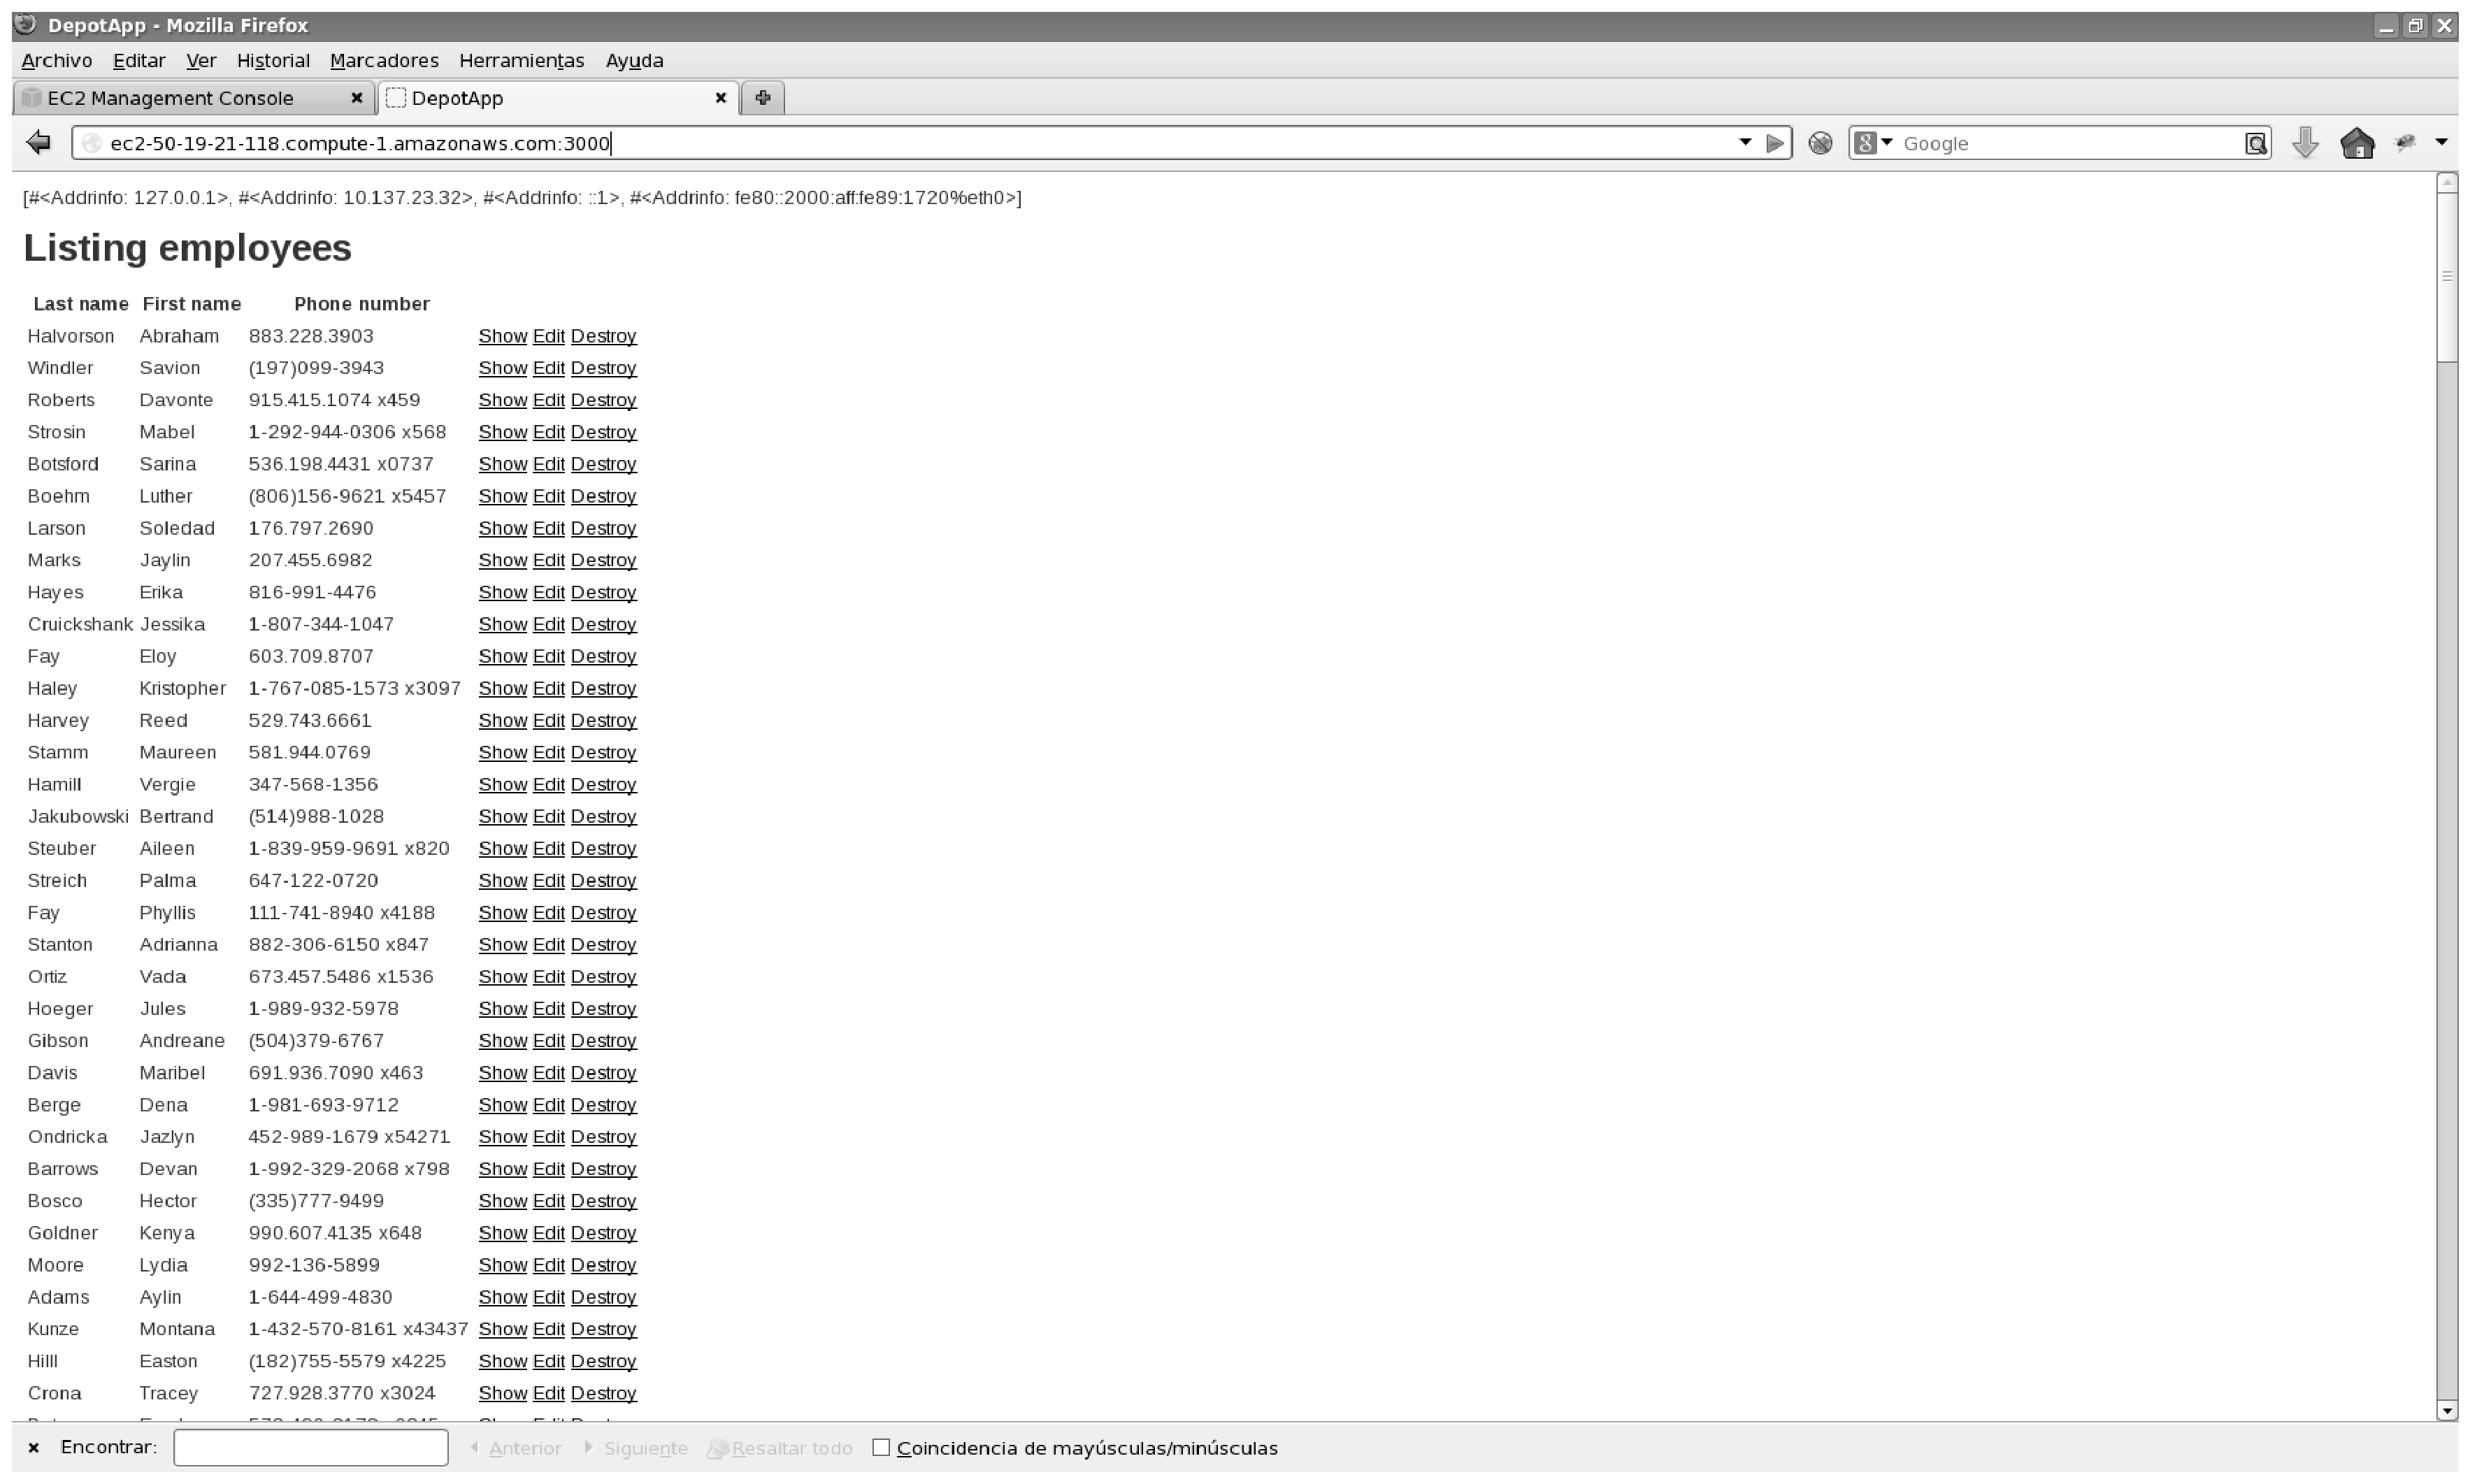
\includegraphics[width=0.75 \textwidth]{tienda.eps}
\end{itemize}
\end{frame}

\section{Application in Developent and Production Environments}
\begin{frame}[fragile, allowframebreaks]
\frametitle{Application in Developent and Production Environments}
\begin{itemize}
\item Edit \texttt{config/database.yml} file (configuration database file) in order to run the application with \texttt{PostgreSQ}L instead of sqlite3 database

\lstset{language=Ruby, style=eclipse, numbers=left}
\begin{lstlisting}[escapechar=!]
!\vdots!
production:
  adapter: postgresql
  encoding: unicode
  database: depot_app_production
  pool: 5
  username: depot_app
  password: 123456 # your favorite password
!\vdots!
\end{lstlisting}

\item Create \texttt{depot\_app\_production} database, migrate tables and  seed the data

\lstset{language=shell, style=eclipse}
\begin{lstlisting}[numbers=none, escapechar=!]
$ rake db:create RAILS_ENV=production
$ rake db:migrate RAILS_ENV=production
$ rake db:seed RAILS_ENV=production
\end{lstlisting}

\lstset{language=shell, style=eclipse}
\begin{lstlisting}[escapechar=!]
$ rails server --environment production
\end{lstlisting}

\item Curl the URL of the files you just created

\lstset{language=shell, style=eclipse}
\begin{lstlisting}[escapechar=!]
$ curl http://my.public.dns.amazonaws.com:3000
\end{lstlisting}

Problems? Kill Webrick server and export the ``assests''. 

\lstset{language=shell, style=eclipse}
\begin{lstlisting}[escapechar=!]
$ rake assets:precompile RAILS_ENV=production
$ rails server --environment production
\end{lstlisting}

\item Curl the URL of the files you just created. It works!
\lstset{language=shell, style=eclipse}
\begin{lstlisting}[escapechar=!]
$ curl http://my.public.dns.amazonaws.com:3000
\end{lstlisting}
\end{itemize}

\end{frame}
%%%%%%%%%%%%%%%%%%%%%%%%%%%%%%%%%%%%%%%%%%%%%%%%%%%%%%%%%%%%%%%%%%%%%%%%%%%%%%
\section{Professional Web Server in Production Environment}
\begin{frame}[fragile]
\frametitle{Professional Web Server in Production Environment}

\begin{tabular}{cl}
 & Webrick \\
 & Mongrel in \href{https://mongrel.rubyforge.org}{https://mongrel.rubyforge.org}\\

\includegraphics[width=0.15 \textwidth]{unicorn.eps} & Unicorn in \href{https://github.com/depot/517-unicorn}{https://github.com/depot/517-unicorn} \\ 

\includegraphics[width=0.15 \textwidth]{passenger.eps} & Passenger in \href{https://www.phusionpassenger.com/}{https://www.phusionpassenger.com/} \\ 

\includegraphics[width=0.15\textwidth]{thin.eps}  & Thin in \href{https://code.macournoyer.com/thin/}{https://code.macournoyer.com/thin/} \\ 
\end{tabular}


\end{frame}

\subsubsection{Unicorn Configuration}
\begin{frame}[fragile, allowframebreaks]
\frametitle{Unicorn Configuration}

\begin{itemize}
\item  We install the unicorn gem in the gemset

\lstset{language=shell, escapechar=!}
\begin{lstlisting}[escapechar=!]
$ cd ~/public_html/depot_app
$ echo "gem `unicorn`, group:  :production" >> Gemfile
$ bundle install
!\outputcommand{A lot of stuff...}!
\end{lstlisting}

\item To be able to start Unicorn within \acrshort{rvm} environment from an \texttt{init.d} script, we now need to generate a corresponding wrapper

\lstset{language=shell, escapechar=!}
\begin{lstlisting}[escapechar=!]
$ rvm current
$ rvm wrapper ruby-2.0.0-p353@railstutorial_rails_4_0 bootup unicorn
!\outputcommand{Regenerating 2.0.0 wrappers}!
\end{lstlisting}

\item Download \href{https://github.com/defunkt/unicorn/blob/master/examples/unicorn.conf.rb}{https://github.com/defunkt/unicorn/blob/master/examples/unicorn.conf.rb}
and save as \texttt{config/unicorn.rb}. Then edit the unicorn configuration file \texttt{config/unicorn.rb}

\lstset{language=Ruby, style=eclipse}
\begin{lstlisting}[escapechar=!]
# config/unicorn.rb
# !\circled{1}!
# https://github.com/defunkt/unicorn/blob/master/examples/unicorn.conf.rb
!\vdots!
# user "unprivileged_user", "unprivileged_group"
# !\circled{2}!
user "depot_app", "depot_app"

# Help ensure your application will always spawn in the symlinked
# "current" directory that Capistrano sets up.
# !\circled{3}!
# working_directory "/path/to/app/current" # available in 0.94.0+
APP_PATH = "/home/depot_app/public_html/depot_app"
working_directory APP_PATH # available in 0.94.0+

# listen on both a Unix domain socket and a TCP port,
# we use a shorter backlog for quicker failover when busy
# !\circled{4}!
# listen "/path/to/.unicorn.sock", :backlog => 64
listen "/tmp/.unicorn_depot_app.sock", :backlog => 64
listen 8080, :tcp_nopush => true

# nuke workers after 30 seconds instead of 60 seconds (the default)
timeout 30

# feel free to point this anywhere accessible on the filesystem
# !\circled{5}!
# pid "/path/to/app/shared/pids/unicorn.pid"
pid "/var/run/unicorn_depot_app.pid"

# By default, the Unicorn logger will write to stderr.
# Additionally, ome applications/frameworks log to stderr or stdout,
# so prevent them from going to /dev/null when daemonized here:
# !\circled{6}!
# stderr_path "/path/to/app/shared/log/unicorn.stderr.log"
# stdout_path "/path/to/app/shared/log/unicorn.stdout.log"
stderr_path APP_PATH + "/log/unicorn_depot_app.stderr.log"
stdout_path APP_PATH + "/log/unicorn_depot_app.stdout.log"
!\vdots!                                                                      
\end{lstlisting}

\item Run Unicorn Server in production mode

\lstset{language=shell, style=eclipse}
\begin{lstlisting}[escapechar=!]
$ unicorn -E production -p 3000
\end{lstlisting}

\begin{block}{Warning!}
  localhost is ``perdidita''
\end{block}

\item Then run \texttt{curl} in your \alert{localhost} in order to test it

\begin{lstlisting}[escapechar=&]
$ curl http://my.public.dns.amazonaws.com:3000
\end{lstlisting}

\end{itemize}



\end{frame}


%%%%%%%%%%%%%%%%%%%%%%%%%%%%%%%%%%%%%%%%%%%%%%%%%%%%%%%%%%%%%%%%%%%%%%%%%%%%%%
\subsubsection{Unicorn Init Script}
\begin{frame}[fragile, allowframebreaks]
\frametitle{Writing an Unicorn Init Script}
\begin{itemize}
\item Create and start the init script \texttt{/etc/init.d/unicorn\_depot\_app} with port number \texttt{\alert{5000}}
\lstset{language=shell, escapechar=!}
\begin{lstlisting}[escapechar=!]
#/bin/bash

### BEGIN INIT INFO
# Provides:             unicorn
# Required-Start:       $remote_fs $syslog
# Required-Stop:        $remote_fs $syslog
# Default-Start:        2 3 4 5
# Default-Stop:         0 1 6
# Short-Description:    Unicorn webserver
# Description:          Unicorn webserver for depot_app
### END INIT INFO

UNICORN=/home/depot_app/.rvm/bin/bootup_unicorn
UNICORN_ARGS="-D -c /home/depot_app/public_html/depot_app/config/unicorn.rb -p 5000 -E production"
KILL=/bin/kill
PID=/var/run/unicorn_depot_app.pid

sig() {
  test -s "$PID" && kill -$1 `cat $PID`
}

case "$1" in
  start)
    echo "Starting unicorn..."
    $UNICORN $UNICORN_ARGS
    ;;
  stop)
    echo "Stoping unicorn..."
    sig QUIT && exit 0
    echo >&2 "Not running"
    ;;
  restart)
    $0 stop
    $0 start
    ;;
  status)
    ;;
  *)
    echo "Usage: $0 {start|stop|restart|status}"
esac
\end{lstlisting}

\lstset{language=shell, escapechar=!}
\begin{lstlisting}[escapechar=!]
# chmod +x /etc/init.d/unicorn_depot_app
# /etc/init.d/unicorn_depot_app start
# chkconfig unicorn_depot_app on
# chkconfig --list unicorn_depot_app
\end{lstlisting}

\begin{block}{Warning!}
  localhost is ``perdidita''
\end{block}

\item Then run \texttt{curl} in your \alert{localhost} in order to test it

\begin{lstlisting}[escapechar=&]
$ curl http://my.public.dns.amazonaws.com:5000
\end{lstlisting}


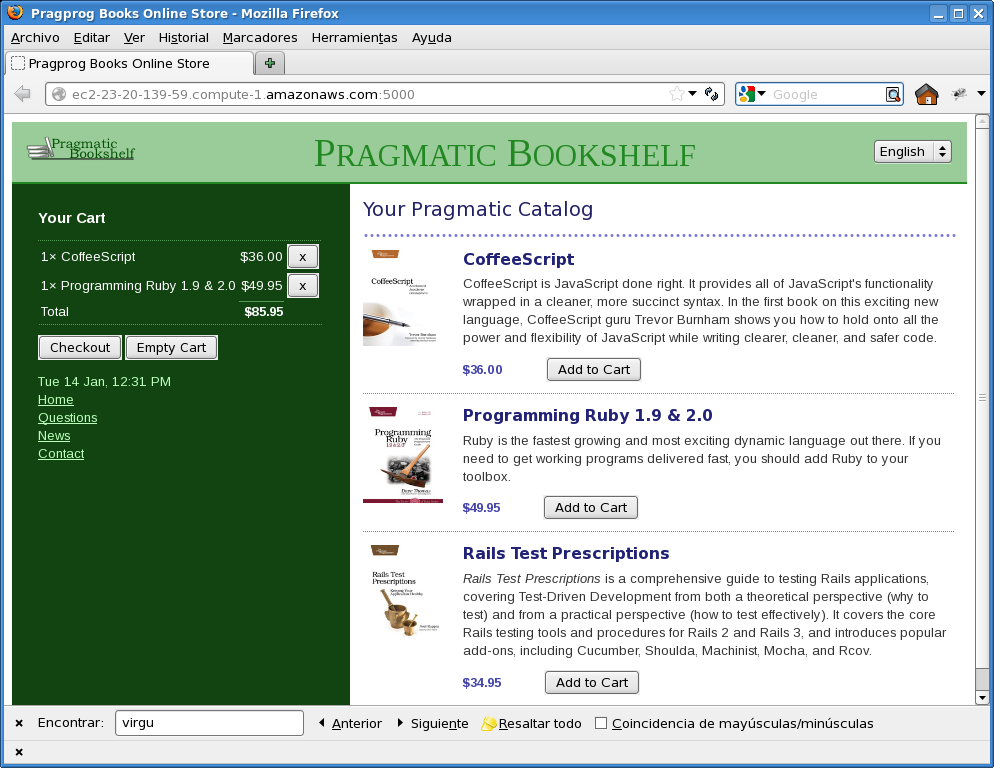
\includegraphics[width=0.6 \textwidth]{tienda5000.eps}

\end{itemize}

\end{frame}

%%%%%%%%%%%%%%%%%%%%%%%%%%%%%%%%%%%%%%%%%%%%%%%%%%%%%%%%%%%%%%%%%%%%%%%%%%%%%%
\subsubsection{Adding a Virtual Host}
\begin{frame}[fragile, allowframebreaks]
\frametitle{Adding a Virtual Host}
\begin{itemize}
 \item  Add a Virtual Host in Apache configuration file \texttt{/etc/httpd/conf/httpd.conf}

\lstset{language=shell, escapechar=&, numbers=left}
\begin{lstlisting}
&\vdots&
&\circled{1}&
NameVirtualHost *:80
&\vdots&
&\circled{2}&
<VirtualHost *:80>
  ServerAdmin webmaster@blog_app.com
  DocumentRoot /home/deployer/blog_app
  ServerName blog_app.com
  ErrorLog logs/blog_app.example.com-error_log
  CustomLog logs/blog_app.example.com-access_log common

  RewriteEngine On

# Redirect all non-static requests to unicorn
  RewriteCond %{DOCUMENT_ROOT}/%{REQUEST_FILENAME} !-f 
  RewriteRule ^/(.*)$ http://127.0.0.1:5000%{REQUEST_URI} [P,QSA,L]
</VirtualHost>
\end{lstlisting}

\item Add to the file \texttt{/etc/hosts}
\lstset{language=shell, escapechar=&}
\begin{lstlisting}
# echo "my.public.dns.amazonaws.com depot_app depot_app.com >> /etc/hosts" 
\end{lstlisting}

\item Restart Apache daemon

\lstset{language=shell, escapechar=!}
\begin{lstlisting}[escapechar=!]
# /etc/init.d/httpd restart
\end{lstlisting}

\item Curl the URL just created

\begin{lstlisting}[escapechar=!]
$ curl http://depot_app.com
\end{lstlisting} 

\end{itemize}

\end{frame}

%%%%%%%%%%%%%%%%%%%%%%%%%%%%%%%%%%%%%%%%%%%%%%%%%%%%%%%%%%%%%%%%%%%%%%%%%%%%%%
\section{Homeworks}
\begin{frame}
  \frametitle{Homeworks}
  \begin{itemize}
    \item Deployment a Rails Application with Mongrel, Passenger or Thin
    \item Start Up PhpPgAdmin tool
    \item Deployment your favorite Content Manager System (Joomla!, Drupal \dots in Amazon)
  \end{itemize}
\end{frame}

\end{document}

\begin{frame}
  \frametitle{Glossary}
  % \printglossary
\end{frame}

